\documentclass[a4paper,10pt]{scrartcl}
\usepackage{physik-vorlesung}

\title{Physik Vorkurs}

\begin{document}

\maketitle

\tableofcontents
\newpage
\section{Grundlagen}
\subsection{Was ist Physik}
\begin{seg}{(Versuch einer Definition)}
 Physik ist eine \emph{Naturwissenschaft}, die sich mit der \emph{rationalen Beschreibung} von Naturerscheinungen mit der Untersuchung der \emph{Ursachen und Wirkungen}.
\end{seg}
\begin{seg}{Grundprinzipien}

\begin{description}
 \item[WIE?] Naturwissenschaft $\longrightarrow$ Methode
 \item[WAS?] rationale Beschreibung $\longrightarrow$ Unterteilung
 \item[WARUM?] Ursachen und Wirkungen $\longrightarrow$ Zusammenhang der Gesetze, Reproduzierbarkeit
\end{description}
\end{seg}

\subsubsection{Gegenstand der Physik}
\begin{seg}{klassische Unterteilung:} 
 Mechanik, E-Lehre, Thermodynamik, etc.
\end{seg}
\begin{ex*} \emph{Blitz}
 \begin{itemize}
  \item Funkentladung: $20000 A$
  \item Erhitzung der Luft: $T \approx 30000 K$
  \item Schall: Druck
  \item B-Feld
 \end{itemize}

\end{ex*}

\begin{enumerate}
 \item Behandle jedes Phänomen als unabhängig
 \item Zusammenhänge: der hypothetisch-deduktive Ansatz
\begin{enumerate}
 \item Beschreibung
 \item Hypothesenfindung
 \item Deduktion
 \item Experiment
\end{enumerate}

\end{enumerate}

\begin{merke}
 Dieses Verfahren hat ausschließlich eine Provisorische Gültigkeit und liegt in der Regel einem Veränderungsprozess zu Grunde.
\end{merke}

\begin{ex} Newtonsche Gravitationsgesetze

 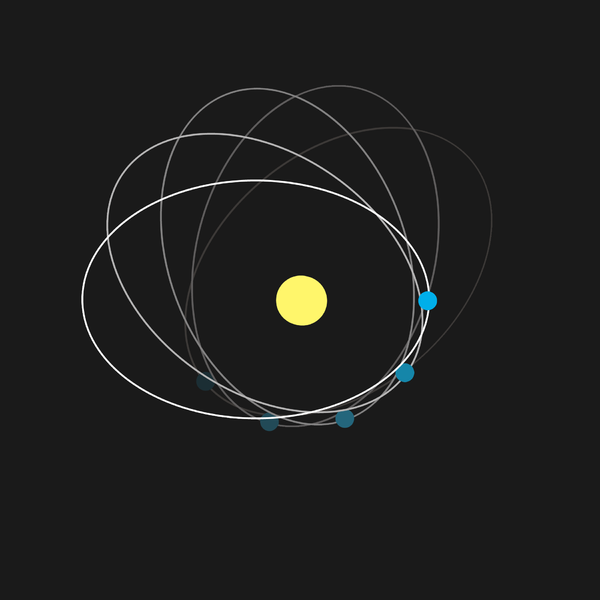
\includegraphics[scale=0.1]{apsidendrehung.png}
\emph{Apsiden- oder Periheldrehung}

Unter einer Apsidendrehung versteht man die Drehung der Ellipsenbahn eines Planeten, dieser lässt sich teilweise durch die Newtonsche Gravitationsgesetze bestimmen zu:

\begin{tabular}{l c r}
Venus & $\rightarrow$ & $280''$ \\
Jupiter & $\rightarrow$ & $150''$ \\
Planeten & $ \rightarrow$ & $100''$ \\
Beschreibung & $\rightarrow$ & $571,91''$
\end{tabular}

Es ergibt sich eine Diskrepanz von $43''$.  Unter Einbeziehung der \emph{allgemeinen Relativitätstheorie} verbleibt eine Diskrepanz von $42''$.  Die Newtonsche Gravitationsgesetze reichen nicht aus, um die \emph{Anomalie} zu beschreiben.
\end{ex}

\subsection{Physikalische Gesetze}
Eine \emph{physikalische Größe}  ist eine quantitative bestimmte Eigenschaft eines  physikalischen Objekts.

Sie besitzt einige charakteristische Eigenschaften:
\begin{itemize}
 \item Maßvorschrift: 
\subitem $\mapsto$ direkt [Bsp.: Meterstab]
\subitem $\mapsto$ geeichtes Instrument [Bsp.: Federwage]
\subitem $\mapsto$ indirekt [Bsp.: Flächeninhalt Dreieck] 
 \item Messaparatur
 \item Einheit:  $G=\underbrace{\{G\}}_{\text{Maßzahl}}\underbrace{[G]}^{\text{Einheit}}=n\cdot U_G$
\end{itemize}
\begin{ex} Grundgrößen der Mechanik
\begin{table}[h]
\begin{tabular}{l c c l}
 Größe:  &   Anwendung: & Einheit & Messaparatur\\
 1) Länge: &  Raummessung & \textbf{m} & Meterstab\\
 2) Zeit: & Abfolge von Ereignissen & \textbf{s} & Uhr\\
 3) Masse: & Eigenschaft der Materie & \textbf{kg} & Waage
\end{tabular}
\end{table}

Länge und Zeit bilden hierbei die \emph{Kinematik}.  Länge, Zeit und Masse stellen die \emph{Dynamik} dar.
\end{ex}

\subsubsection{Dimension und Einheit}
$G=L^\alpha M^\beta T^{\gamma}$, $\alpha$, $\beta$ und $\gamma$ bezeichnet man als die \emph{Dimensionen} der Grundgrößen der Mechanik $L, M, T$.
\begin{note}
 In der Regel arbeitet man mit ganzzahligen Dimensionen.
\end{note}

\begin{ex}

\begin{itemize}
 \item \emph{Fläche} $[A]=[L^2 M^0 T^0]=[L^2]$
 \item \emph{Volumen} $[V]=[L^3M^0T^0]=[L^3]$
 \item \emph{Geschwindigkeit} $[v]=[L^1M^0T^{-1}]=[L^1 T^{-1}]$
\end{itemize}
Hiermit stellen \emph{Fläche} und \emph{Volumen} kinematische und die \emph{Geschwindigkeit} dynamische Größen dar.
\end{ex}
\newpage  
\begin{seg}{Methode: Umrechnung}
 Seien $G=n_1\cdot U_{1L}^\alpha U_{1M}^\beta U_{1T}^\gamma$ und $G=n_2\cdot U_{2L}^\alpha U_{2M}^\beta U_{2T}^\gamma$ Darstellungen von $G$.
 \[
  \implies n_2=n_1 \cdot \left ( \frac{U_{1L}}{U_{2L}} \right )^\alpha \left ( \frac{U_{1M}}{U_{2M}} \right )^\beta \left ( \frac{U_{1T}}{U_{2T}} \right )^\gamma
 \]
\end{seg}
\begin{ex}
 Bestimmung des Flächeninhalts eines Rechtecks der Größe $10 \text{cm} \times 1\txt{cm}$.  Der Inhalt ergibt sich also zu $A=10\text{cm}\cdot 1 \text{cm}=10\txt{cm}^2=x\txt{m}^2$.  Berechne $x$.
\[
 x=10 \left ( \frac{1 \txt{cm}}{1 \txt{m}} \right ) = 10 \left ( \frac{1 \txt{cm}}{100 \txt{cm}} \right )=0,001
\]

\end{ex}

\subsubsection{Messfehler}
\begin{enumerate}
 \item Systematische: $T=\omega \pm \sigma$
 \item statischtische Fehler:\\
 \begin{itemize}
  \item $N$ Messungen
  \item Quadratische Abweichung: $A=\sum_{i=1}^{N}(x-x_i)^2$
\subitem $\mapsto$ Suche Minimum:
\[
 \frac{dA}{dx} \mid_{x=\tilde x}=2 \sum_{i=1}^N(x-x_i) \mid_{x=\tilde x}\stackrel{!}{=}0
\]
\[
  \implies \sum_{i=1}^N x_i=\sum_{i=1}^N \tilde x=N\tilde x \implies \tilde x=\frac{1}{N}  \sum_{i=1}^N x_i
\]


 \end{itemize}

\end{enumerate}








\end{document}